%-------------------------------------------------------------------------------
% seq64_pattern_editor
%-------------------------------------------------------------------------------
%
% \file        seq64_pattern_editor.tex
% \library     Documents
% \author      Chris Ahlstrom
% \date        2015-08-31
% \update      2017-05-13
% \version     $Revision$
% \license     $XPC_GPL_LICENSE$
%
%-------------------------------------------------------------------------------

\section{Pattern Editor}
\label{sec:seq64_pattern_editor}

   The \textsl{Sequencer64 Pattern Editor} is used to edit and preview a
   pattern, as well as to configure its buss and channel settings.

%  In programmer's jargon, this window is represented by the seqroll class (and
%  the other "seq" classes).

\begin{figure}[H]
   \centering 
%  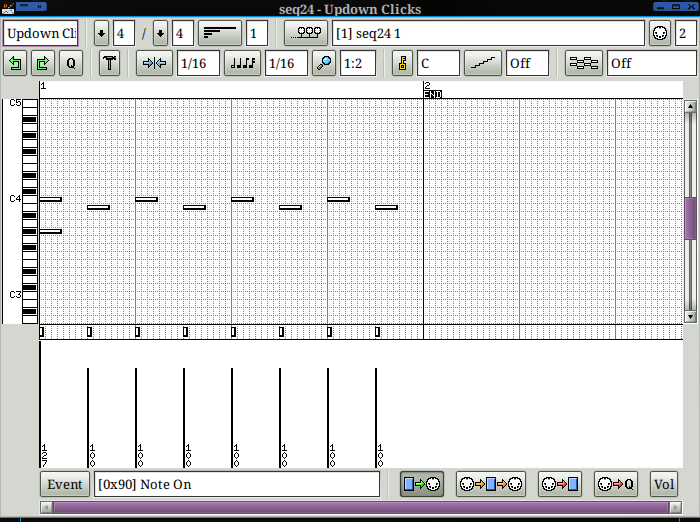
\includegraphics[scale=0.75]{pattern/pattern-edit-window.png}
%  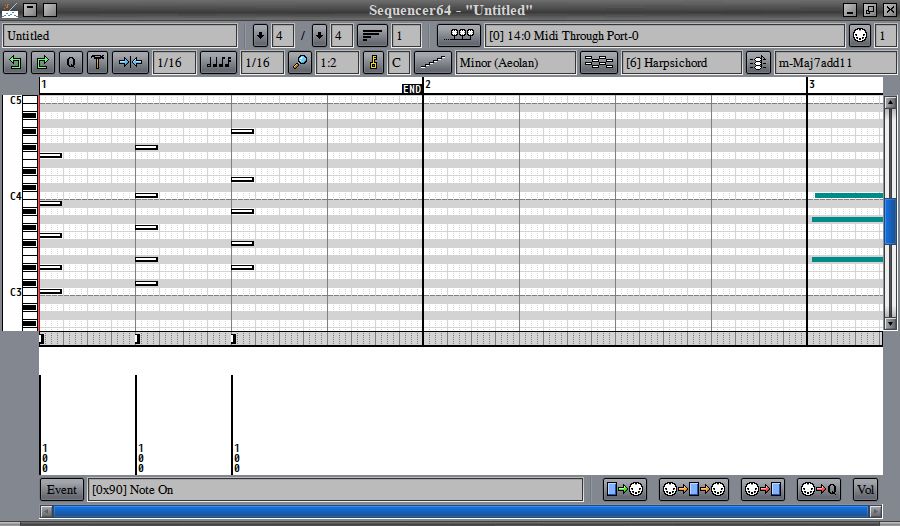
\includegraphics[scale=0.75]{new/pattern_editor_chords-0_9_14.png}
   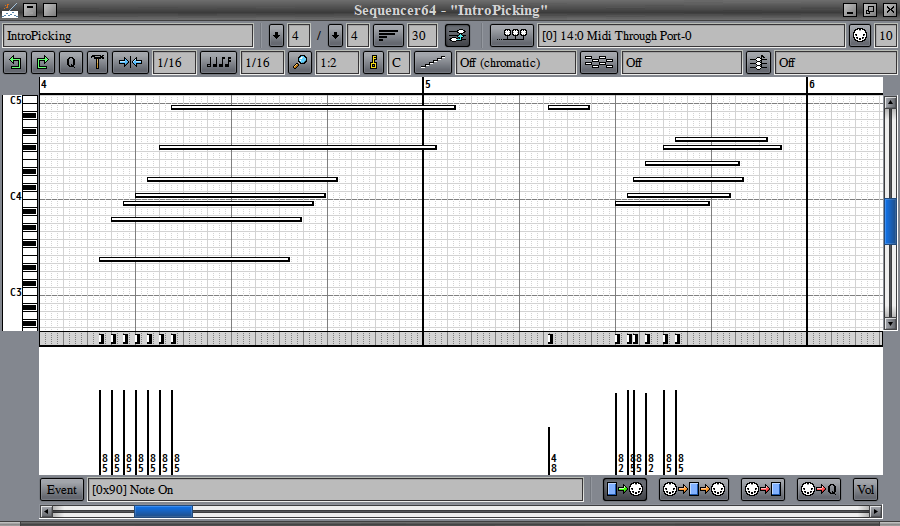
\includegraphics[scale=0.75]{new/pattern_editor_transpose-0_9_15.png}
   \caption{Pattern Edit Window}
   \label{fig:pattern_edit_window}
\end{figure}

   Not shown in this figure are:
   
   \begin{itemize}
      \item The new \textbf{LFO} button in the bottom panel.
      \item The new \textbf{Rec Type} button in the bottom panel,.
   \end{itemize}

   Both are described later, but we need to update the screenshot at some
   point.

   This dialog is complex.
   For exposition, we break it into some common actions, a first panel, a
   second panel, a bottom panel, and a piano-roll/events section.

   \begin{enumber}
      \item \textbf{First Panel}
      \item \textbf{Second Panel}
      \item \textbf{Piano-Roll/Events Panel}
      \item \textbf{Bottom Panel}
      \item \textbf{Common Actions}
   \end{enumber}

   Before we describe this window, there are some things to recognize.
   First, if the pattern is empty when play is started, the progress bar will
   still move.  This is necessary to help the user key in a new pattern.
   Second, to add a note, one must press the right mouse button (the pointer
   changes to a pencil) and, while holding it, press the left mouse button.
   Or, to use a keystroke, click in the pattern editor, press
   \index{keys!p}
   \texttt{p} to select the "pencil" or "paint" mode, then
   \index{mouse!left-click}
   left-click to add a note or
   \index{mouse!left-click-drag}
   left-click-drag to add multiple notes as the mouse moves..
   \index{keys!x}
   Press or release the right mouse button, or press
   \texttt{x} to "eXit" or "eXscape" from that mode.  Also remember
   that notes are drawn only with the length selected by the "notes" button
   near the top of the pattern window.  There are some other tricks to
   modifying the new notes that are described later.

   Also new with \textsl{Sequencer64}, and not in \textsl{Seq24}, is the
   automatic horizontal scrolling of the sequence/pattern editor window when
   playback moves the progress bar outside of the current frame of data.  This
   feature makes it easier to follow patterns that are longer than a measure or
   two.
   
   Note that \textsl{Sequencer64} also provides a way to restart the progress
   bar within the pattern without resetting it to the beginning of the pattern.
   \index{pause} This new feature is called "pause".  It can be accessed by the
   \index{keys!.}
   \index{keys!pause}
   new pause key (which defaults to the period character) or by the pause
   button, which appears when playback is underway.  (Note that this feature
   can be disabled if the application is built via source code.  Also note that
   it works only in ALSA mode at present.)

\subsection{Pattern Editor / First Panel}
\label{subsec:seq64_pattern_editor_first}

   The top bar (horizontal panel) of the Pattern (sequence) Editor
   lets one change the name of
   the pattern, the time signature of the piece, how long the loop is, and
   some other configuration items.

\begin{figure}[H]
   \centering 
   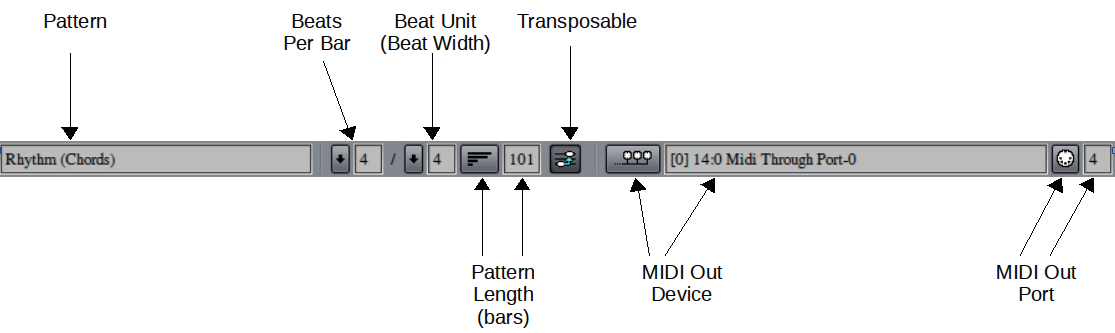
\includegraphics[scale=0.55]{pattern/pattern-edit-first-panel-items.png}
   \caption{Pattern Editor, First Panel Items}
   \label{fig:pattern_editor_first_panel_items}
\end{figure}

   In recent versions of \textsl{Sequencer64}, a "sequence-is-transposable"
   feature has been added, as shown above.

% \begin{figure}[H]
%    \centering 
%    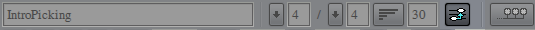
\includegraphics[scale=0.75]{new/pattern_editor_top_panel-0_9_15.png}
%    \caption{Pattern Editor, First Panel Emphasizing Transposable Button}
%    \label{fig:pattern_editor_first_panel_transposable}
% \end{figure}

   \begin{enumber}
      \item \textbf{Pattern Name}
      \item \textbf{Beats Per Bar}
      \item \textbf{Beat Unit (Beat Width)}
      \item \textbf{Pattern Length}
      \item \textbf{Transposable (toggle)}
      \item \textbf{MIDI Out Device}
      \item \textbf{MIDI Out Port}
   \end{enumber}

   \setcounter{ItemCounter}{0}      % Reset the ItemCounter for this list.

   \itempar{Pattern Name}{pattern editor!name}
   Provides the name of the pattern.
   This name should be short and memorable.
   It is displayed in the Patterns window, on the top line of its pattern
   box/slot.
   Unfortunately, there is no edit cursor in this field (not sure why yet), so
   one has to edit blind.

   \itempar{Beats Per Bar}{pattern editor!beats/bar}
   Part of the time signature, and specifies the number of beat units per bar.
   The possible values range from 1 to 16, if the drop-down menu is used.
   As of version 0.90.6, the numeric value can be directly edited, to achieve
   non-standard values, thanks to an update from Jean-Emmanuel.

   \itempar{Beat Unit (Beat Width)}{pattern editor!beat unit}
   \index{pattern editors!beat width}
   \index{beat width}
   Part of the time signature, and specifies the size of the beat unit:
   1 for whole notes; 2 for half notes; 4 for quarter notes; 8 for eight notes;
   16 for sixteenth notes; and 32 for thirty-second notes.
   The whole time signature is display at the bottom center of a pattern
   slot.

   \itempar{Pattern Length}{pattern editor!length}
   Sets the length of the current pattern, in measures.
   The possible values range from 1 to 16, then 32, and 64.
   \textsl{However}, when opening or importing a non-\textsl{Sequencer64}
   MIDI tune, the length of each track will be used, and so other values
   are possible; they just cannot be set via the user-interface.
   However, as of version 0.90.6, the numeric value can be directly edited, to
   achieve non-standard values, thanks to an update from Jean-Emmanuel.

   Note that bringing up a short sequence (one less than one measure or bar in
   length) in the pattern editor will adjust the sequence to pad it to the
   length of one measure.  For example, a sequence containing just one program
   change will be padded to the size of a full measure.
   This adjustment makes it show progress more smoothly in the main window when
   the sequence is playing.
   \index{pattern editor!progress bar}
   \textsl{Sequencer64} will, when it reads such a short sequence
   from a MIDI file (whether foreign or native to \textsl{Sequencer64}),
   pre-pad it to the length of a measure, so that it will always show smooth
   progress.

   It would be nice to have a value that represents
   "indefinite", so that the loop or pattern would be more like a track,
   and not be repeatable.  We have part of that functionality:
   as of version 0.90.5, we have incorporated changes from user
   Stazed that allow the pattern to expand indefinitely while the user inputs
   MIDI from a controller.
   See \sectionref{subsec:seq64_pattern_editor_bottom} below.
   Also nice would be a "one-shot"
   pattern, useful for live intro patterns, for example.)

   \itempar{Transpose Toggle}{pattern editor!transpose toggle}
   This item, if enabled in the build, allows the sequence to be transposed by
   the global transpose selection made in the song editor.  If transpose is
   enabled for that pattern, the button will be highlighted as per the current
   desktop theme.  Patterns for drums should, in general, not be transposable.

   \itempar{MIDI Out Device (Buss)}{pattern editor!midi out device}
   This setting specifies one of the 16 MIDI output busses provided by
   \textsl{Sequencer64}, or one of the MIDI devices set up in the computer.
   The settings look a lot like
   \figureref{fig:pattern_window_right_click_midi_bus}.

   \itempar{MIDI Out Port (Channel)}{pattern editor!midi out port}
   This settings select the MIDI output channel, or port.
   The possible values range from 1 to 16.
   If instruments are defined in the "user" configuration file
   to that device and channel, their names will be shown.

\subsection{Pattern Editor / Second Panel}
\label{subsec:seq64_pattern_editor_second}

   The second horizontal panel of the Pattern Editor provides a number
   of additional settings.

\begin{figure}[H]
   \centering 
   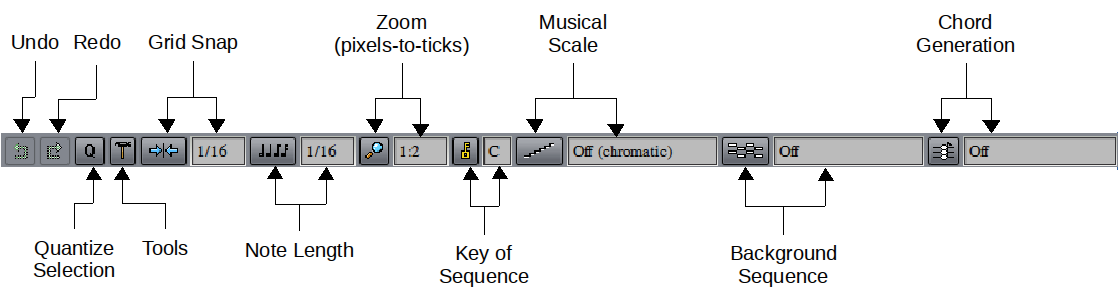
\includegraphics[scale=0.55]{pattern/pattern-edit-second-panel-items.png}
   \caption{Pattern Editor, Second Panel Items}
   \label{fig:pattern_editor_main_panel_items}
\end{figure}

   We show a new screen-shot, because there is a new button to the right
   of the \textbf{Tools} ("hammer" button).  This button toggles the "follow
   progress" feature; it is the active button in the following diagram.

\begin{figure}[H]
   \centering 
   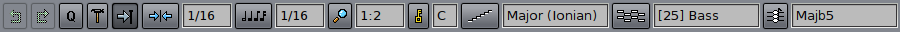
\includegraphics[scale=0.55]{pattern/pattern-edit-second-panel-items-2.png}
   \caption{Pattern Editor, Second Panel Update}
   \label{fig:pattern_editor_main_panel_update}
\end{figure}

   If \textsl{Sequencer64} is built with the new chord-generation option
   built in (the default), then the second panel is wider to make room for an
   addition user-interface item, shown at the right of the figure above.

% \begin{figure}[H]
%    \centering 
%    
\includegraphics[scale=0.75]{new/pattern_editor_second_panel-0_9_14.png}
%    \caption{Pattern Editor, Second Panel Items Emphasizing Chord Button}
%    \label{fig:pattern_editor_main_panel_chord_button}
% \end{figure}

   \begin{enumber}
      \item \textbf{Undo}
      \item \textbf{Redo}
      \item \textbf{Quantize Selection}
      \item \textbf{Tools}
      \item \textbf{Follow Progress} (new)
      \item \textbf{Grid Snap}
      \item \textbf{Note Length}
      \item \textbf{Zoom}
      \item \textbf{Key of Sequence}
      \item \textbf{Musical Scale}
      \item \textbf{Background Sequence}
      \item \textbf{Chord Generation}
   \end{enumber}

   \setcounter{ItemCounter}{0}      % Reset the ItemCounter for this list.

   \itempar{Undo}{pattern editor!undo}
   The Undo button will roll back any changes to the pattern from this
   session.
   It will roll back one change each time it is pressed.
   It is not certain what the undo limit (if any) is, however.
   \index{keys!ctrl-z}
   Pressing \texttt{Ctrl-Z} is the same as using the \textbf{Undo} button.

   \itempar{Redo}{pattern editor!redo}
   The Redo button will restore any undone changes to the pattern from this
   session.
   It will restore one change each time it is pressed.
   It is not certain what the redo limit is, however.
   There is no "Redo" key in the pattern editor.

   \itempar{Quantize Selection}{pattern editor!quantize}
   Pressing this button will quantize the selected events, as per
   the \textbf{Grid Snap} setting.

   \itempar{Tools}{pattern editor!tools}
   This button brings up a nested menu of tools for modifying selected
   events and notes.

   \itempar{Follow Progress}{pattern editor!tools}
   Pressing this button toggles whether or not the progress bar follows
   progress in long patterns.  Turning off this feature is useful when
   one wants to concentrate on the current measure without the paging to
   subsequent measures that occurs with the "follow progess" feature.

\begin{figure}[H]
   \centering 
   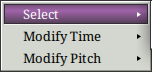
\includegraphics[scale=0.75]{pattern/tools-first-menu.png}
   \caption{Tools, Context Menu}
   \label{fig:pattern_editor_tools_first_menu}
\end{figure}

   \begin{enumber}
      \item \textbf{Select}
      \item \textbf{Modify Time}
      \item \textbf{Modify Pitch}
   \end{enumber}

   $\bullet$ \textbf{Select} provides two sets of selections for notes:
   \begin{itemize}
      \item \textbf{All Notes}, which selects all notes in the pattern;
         Note that \index{keys!ctrl-a} \texttt{Ctrl-A} will also select
         all of the events in the pattern editor.
      \item \textbf{Inverse Notes}, which inverts the selection of notes.
   \end{itemize}

   Other event-selection actions are provided using the mouse in the piano roll:

   \begin{itemize}
      \item \index{mouse!left-click}
         \textbf{Left Click}.
         Pressing the left button on a note or a event deselects all other
         notes or events, and selects the item clicked on.
      \item \index{mouse!ctrl-left-click}
         \textbf{Ctrl Left Click}.
         Pressing the \texttt{Ctrl} key and the left button on a note or an
         unselected event \textsl{adds} that event to the selection.
      \item \index{mouse!left-click-drag}
         \textbf{Left Click Drag}.
         Pressing the left mouse button and dragging also lets one
         select ("lasso") multiple events and notes.
      \item \index{mouse!ctrl-left-click-drag}
         \textbf{Ctrl Left Click Drag}.
         \begin{itemize}
            \item Pressing the \texttt{Ctrl} while left-click-dragging
               \textsl{on unselected events} lets one make additional
               selections of multiple events and notes.
            \item Pressing the \texttt{Ctrl} while left-click-dragging
               \textsl{on an already-selected event} lets one stretch or
               compress the lengths of multiple notes in the selection.
         \end{itemize}
   \end{itemize}

   There are many things that can be done with selected notes, as will be seen
   in the following paragraphs.

   \index{modify event-data}
   $\bullet$ \textbf{Modify Event Data} offers a way to change the event data
   (the lower pane of the pattern editor, the "data pane").
   By left-dragging the mouse in the data pane across the value lines that are
   shown, the values are chopped or set to the height of the mouse pointer at
   each event.
   When notes are selected, and the
   mouse is used to change the values (heights) of the lines in the event-data
   area,
   \textsl{only the events that are selected} are changed.  The data-values of
   \textsl{unselected} events are left unchanged.
   A cool feature from \textsl{Seq24}.

   \index{modify time}
   $\bullet$ \textbf{Modify Time} offers two ways to tweak the timing of the
   selected note:
   \index{quantize}
   \textbf{Quantize Selected Notes}, which quantizes the selected
   notes, the same way as the \textbf{Quantize} ("\textbf{Q}") button;
   \index{tighten}
   \textbf{Tighten Selected Notes}, which is merely a less
   strict form of quantization.

   \index{modify pitch}
   $\bullet$ \textbf{Modify Pitch} has only one entry by default,
   \textbf{Transpose Selected} (not shown).
   Selecting the \textbf{Transpose Selected} entry
   brings up the following sub-menu:

\begin{figure}[H]
   \centering 
   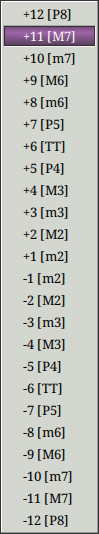
\includegraphics[scale=0.75]{pattern/tools-transpose-selected-menu.png}
   \caption{Tools, Transpose Selected Values}
   \label{fig:pattern_editor_tools_transpose_selected_menu}
\end{figure}

   $\bullet$ If the user has selected a
   \textbf{Musical Scale} setting other than \textbf{Off},
   then \textbf{Modify Pitch} has two entries:
   \textbf{Transpose Selected}, discussed above, plus
   another sub-menu,
   \textbf{Harmonic Transpose Selected}, which makes sure that all
   transpositions stay on the selected scale.

   Note that one can also modify the pitch of selected notes by the
   \index{mouse!left-click-drag}
   left-click-drag action, or by moving the selection using the
   \index{keys!down-arrow}
   \index{keys!up-arrow}
   up-arrow or down-arrow keys.

\begin{figure}[H]
   \centering 
   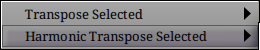
\includegraphics[scale=0.75]{pattern/tools-transpose-and-harmonic-selected-menu.png}
   \caption{Tools, Two "Transpose" Menus}
   \label{fig:pattern_editor_tools_two_transpose_menus}
\end{figure}

   Remember that only the \textbf{Transpose Selected} entry is shown if the
   \textbf{Musical Scale} setting is \textbf{Off}.
   Selecting the \textbf{Harmonic Transpose Selected} entry brings up the
   following sub-menu:

\begin{figure}[H]
   \centering 
   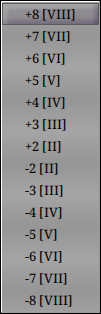
\includegraphics[scale=0.75]{pattern/tools-harmonic-transpose-selected-menu.png}
   \caption{Tools, Harmonic Transpose Selected Values}
   \label{fig:pattern_editor_tools_harmonic_transpose_menu}
\end{figure}

   Again, the harmonic-transpose option will not be available unless a scale
   has been selected.

   \itempar{Grid Snap}{pattern editor!grid snap}
   Grid snap selects where the notes will be drawn.
   The following values are supported:
   1, 1/2, 1/4, 1/8, 1/16, 1/32, 1/64, and 1/128.
   Additional values are also supported:
   1/3, 1/6, 1/12/, 1/24, 1/48, 1/96, and 1/192.

   \itempar{Note Length}{pattern editor!note length}
   Note Length determines the duration of the inserted notes.
   Like the \textbf{Grid Snap} values,
   the following values are supported:
   1, 1/2, 1/4, 1/8, 1/16, 1/32, 1/64, and 1/128.
   Additional values are also supported:
   1/3, 1/6, 1/12/, 1/24, 1/48, 1/96, and 1/192.

   \itempar{Zoom}{pattern editor!zoom}
   Zoom is the relation between MIDI pixels and ticks, written as
   "pixels:ticks", where "ticks" is really the "pulses" in "PPQN".
   For example, 1:4 = 4 ticks per pixel.
   Supported values are 1:1, 1:2, 1:4, 1:8, 1:16, and 1:32, along with
   more new values to support higher PPQN tunes: 1:64, 1:128, 1:256, and
   1:512.
   The default zoom is 2 for the standard PPQN value, 192, but it
   increases for higher PPQN values.
   This is the zoom of the Pattern Editor.  As the right number goes higher,
   the effect is to zoom out, and show more of the pattern at once.
   In fact, it is probably better to list them as ticks (pulses) per pixel:

   \begin{itemize}
      \item 1 pulse per pixel
      \item 2 pulses per pixel (default value)
      \item 4 pulses per pixel
      \item 8 pulses per pixel
      \item 16 pulses per pixel
      \item 32 pulses per pixel (same as Song Editor)
      \item . . .
      \item 512 pulses per pixel
   \end{itemize}

   \textbf{New:}
   \index{new!zoom keys}
   \index{keys!0}
   \index{keys!z}
   \index{keys!shift-z}
   After one has left-clicked in the piano roll, the "z", "Z", and "0"
   can be used to zoom the piano-roll view.  The "z" key zooms out, the "Z" key
   zooms in, and the "0" key resets the zoom to the default value.
   The zoom feature also modifies the time-line (measures indicator) and
   the data area.
   If, for some reason, the data area and piano-roll get out of sync, click on
   the horizontal scroll bar to force the views to redraw properly.

   \index{song editor!zoom}
   Note that the Song Editor, which now has zoom functionality (through
   the "z", "Z", and "0" keystrokes only),
   has a default resolution of 32 pulses per pixel, so, by default, it has
   16 times the resolution of the Pattern Editor.

   \itempar{Key of Sequence}{pattern editor!key}
   Selects the desired key for the pattern.  The following scales are
   supported:  C, C\#, D, D\#, E, F, F\#, G, G\#, A, A\#, and B.
   Note that changing the \textbf{Key} will also shift the marked notes
   for the \textbf{Musical Scale} setting.

   \textbf{New:}
   \index{new!save musical key}
   As of version 0.9.9.8, the key that a sequence is set to is
   now saved in the MIDI file along with the rest of the data for the sequence.
   \textbf{However},
   it turns out that a change made to the key, scale, or background sequence in
   the sequence editor is saved in that editor, so that opening another sequence
   will apply the same settings to that sequence.  This is an optional feature,
   now more rigorously supported, as noted below.

   \index{global-sequence}
   If the global-sequence-feature is enabled, and the user selects
   a different key, scale, or background sequence in the sequence editor, 
   then \textsl{all} sequences will share the selected key, scale, or background
   sequence.  Furthermore, these settings are saved in the "proprietary"
   section of the MIDI file, where they are available for all sequences.

   If the global-sequence-feature is \textsl{no}t enabled, and the user selects
   a different key, scale, or background sequence in the sequence editor, 
   then only that sequence will use the selected key, scale, or background.
   The key, scale, or background sequence change will be saved in the MIDI file
   only for that sequence, as a SeqSpec meta event.
   The global-sequence-feature setting can be made in the "user" configuration
   file.

   \itempar{Musical Scale}{pattern editor!scale}
   Selects the desired scale for the pattern.
   When a scale is selected, the following features are supported:

   \begin{itemize}
      \item The notes that are \textsl{not}
         in the scale are shown as grey in the piano
         roll, to make it easier to key all notes in-scale.
      \item When harmonic transposition is performed, the notes are shifted
         so that they remain in the selected scale.
      \item The exact notes that are considered "in-scale" depend also on the 
         exact value of the \textbf{Key of Sequence} setting.
   \end{itemize}

   \textbf{New:}
   \index{new!musical scales}
   Originally, only the following scales were supported: Off, Major, and Minor.
   Now, the following scales are supported:

   \begin{itemize}
      \item \textbf{Off (Chromatic)}
      \item \textbf{Major (Ionian)}
      \item \textbf{Minor (Aeolian)}
      \item \textbf{Harmonic Minor}
      \item \textbf{Melodic Minor}
      \item \textbf{Whole Tone}
      \item \textbf{Blues}
      \item \textbf{Major Pentatonic}
      \item \textbf{Minor Pentatonic}
   \end{itemize}

   Please let us know of any mistakes found in the new scales.
   Also please note that the \textbf{Melodic Minor} scale is supposed to
   descend in the same was as the natural \textbf{Minor} scale, but
   there is no way to support that trick in
   \textsl{Sequencer64}.

\begin{figure}[H]
   \centering 
%  \includegraphics[scale=0.75]{pattern/scales-menu.png}
   \includegraphics[scale=1.0]{new/scales-menu.png}
   \caption{Scales Currently Supported in Sequencer64}
   \label{fig:pattern_editor_available_scales}
\end{figure}

   One can select which \textbf{Musical Scale} and
   \textbf{Key} the piece is in,
   and \textsl{Sequencer64} will grey those keys on the piano-roll that
   are \textsl{not} in the selected scale for the selected key.
   This is purely a visual thing; a user can still add off-key notes.
   This effect is shown for the C Major scale in the following figure:

\begin{figure}[H]
   \centering 
   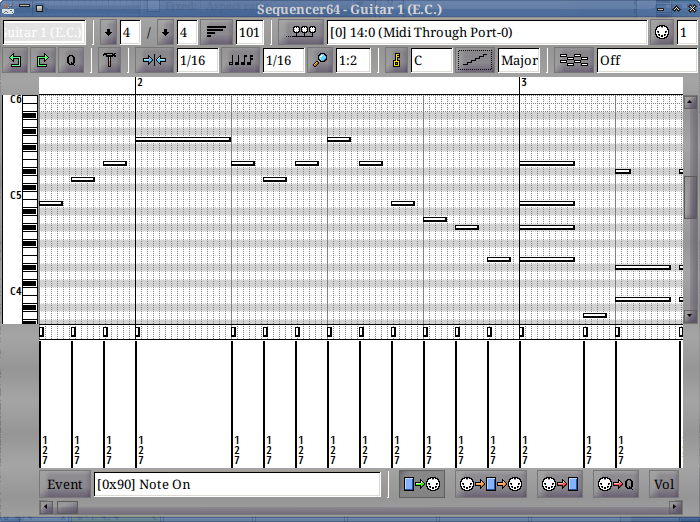
\includegraphics[scale=0.75]{pattern/major-scale-masking.png}
   \caption{C Major Scale Masking}
   \label{fig:pattern_editor_major_scale_masking}
\end{figure}

   This feature makes it a bit easier to stay in key while playing and
   recording.  Note that the scale will shift when a different
   \textbf{Key} is selected.

   \textbf{New:}
   \index{new!save musical scale}
   The scale that a sequence is set to is
   now saved in the MIDI file along with the rest of the data for the sequence.
   \textbf{However},
   it turns out that a change made to the key, scale, or background sequence in
   the sequence editor is saved in the editor, so that opening another sequence
   will apply the same settings to that sequence.  This is a feature.
   The feature had some quirks, which are fixed, and it is now
   an optional feature.
   Also, the user has the option of applying the key/scale/background-sequence
   either globally (all sequences) or locally, per-sequence, with each sequence
   holding its key, scale, and background-sequence settings in
   SeqSpec meta events.

   \itempar{Background Sequence}{pattern editor!background sequence}
   One can select another pattern to draw on the background to help with
   writing corresponding parts.
   The button brings up a small menu with values of \textbf{Off} and
   \textbf{[0]}.  The 0 is a set number. Sets are numbered from 0 to 31.
   Additional set numbers appear in the menu for each set that has data in it.
   Under the \textbf{0}
   entry, a menu like the following appears:

\begin{figure}[H]
   \centering 
   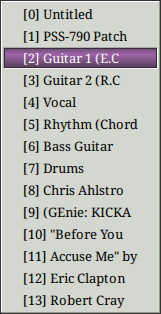
\includegraphics[scale=0.75]{pattern/background-sequence-menu.png}
   \caption{Sample Background Sequence Values}
   \label{fig:pattern_editor_background_sequence_menu}
\end{figure}

   Once the desired pattern is selected from that list, it appears as dark cyan
   note bars, along with the normal notes that are part of the pattern.  (Also
   note the orange selected notes and events in the following figure.)

\begin{figure}[H]
   \centering 
   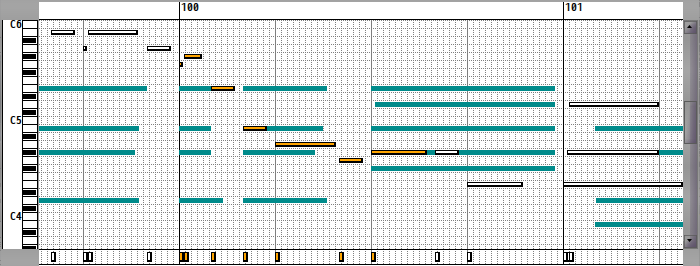
\includegraphics[scale=0.75]{pattern/background-sequence-notes.png}
   \caption{Background Sequence Notes}
   \label{fig:pattern_editor_background_sequence_notes}
\end{figure}

   The dark cyan notes shown represent the rhythm pattern that was selected as
   the background pattern.

   \textbf{New:}
   \index{new!save background seqeuence}
   The background sequence that a sequence shows is saved in the MIDI file
   along with the rest of the data for the sequence.
   \textbf{However},
   it turns out that a change made to the key, scale, or background sequence in
   the sequence editor is saved in the editor, so that opening another sequence
   will apply the same settings to that sequence.  This is an optional feature,
   now more rigorously supported, as noted earlier.

   \itempar{Chord Generation}{pattern editor!chord generation}
   The ability to insert chords with one click has been added.
   This feature comes from user "stazed"
   and his \textsl{Seq32} project (\cite{seq32}).

\begin{figure}[H]
   \centering 
   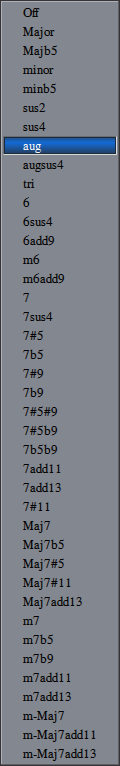
\includegraphics[scale=1.0]{new/chords_menu-0_9_14.png}
   \caption{Chord Generation Menu}
   \label{fig:pattern_editor_chords_menu}
\end{figure}

   The figure shows the menu broken into two pieces.
   Once a value other than \textbf{Off} is selected, a left-click
   in drawing mode will add multiple notes representing the chord
   created, with the clicked note value as the base of the chord.

\subsection{Pattern Editor / Piano Roll}
\label{subsec:seq64_pattern_editor_piano_roll}

   The piano roll is the center of the pattern (loop, track, sequence) editor.
   It is accompanied by a
   \index{event area}
   thin "event bar" (or "event area", or "event strip") just below it,
   \index{data area}
   and a taller "data bar" or "data area" just below that.  While the pattern
   editor is very similar to note editors in other sequencers, it is a bit
   different in feel.  A good mouse with 3 or more buttons is practically a
   necessity for editing (though we have made \textsl{Sequencer64} more usable
   with some crummy trackpads now common on modern laptops, and also usable
   with keystrokes.) We tend to like the Logitech Marble Mouse, an ambidextrous
   USB trackball.  It has four buttons, and we use the
   \texttt{contrib/scripts/marblemouse} script to set up the left small button
   as a middle button.  The script merely makes the following call:

   \begin{verbatim}
      xmodmap -e "pointer = 1 8 3 4 9 6 7 2 5 10 11"
   \end{verbatim}

   Editing is much easier after making that setting.   Of course, keystrokes
   and additional mouse configuration have been added to make editing easier
   even without a good mouse.
   For example, one can page up and down vertically in the piano roll using the
   \index{keys!page-up} Page Up and 
   \index{keys!page-down} Page Down keys.
   One can go to the top using the 
   \index{keys!home} Home key, and
   to the bottom using the
   \index{keys!end} End key.
   One can page left and right horizontally in the piano roll using the
   \index{keys!shift-page-up} Shift Page Up and 
   \index{keys!shift-page-down} Shift Page Down keys.
   One can go to the leftmost position using the 
   \index{keys!shift-home} Home key,
   and to the rightmost position using the
   \index{keys!shift-end} End key,
   And there are more keystroke actions to be described later.

   \index{step}
   \index{note step}
   Also, do not forget the note-step option.  If one paints notes with the mouse,
   the note is previewed, and the note position advances with each click.  If
   one paints notes via an external MIDI keyboard, the notes are painted and
   advanced, but they are not previewed.  To preview them, click the
   \textbf{pass MIDI in to output} button to activate so that they will be
   passed to one's sound generator or software synthesizer.

\subsubsection{Pattern Editor / Piano Roll Items}
\label{subsubsec:seq64_pattern_editor_piano_roll_items}

   The center of the pattern editor consists of a time panel at the top,
   a virtual keyboard at the left, a note grid, a vertical scrollbar, an event
   panel, and a data panel at the bottom.

\begin{figure}[H]
   \centering 
   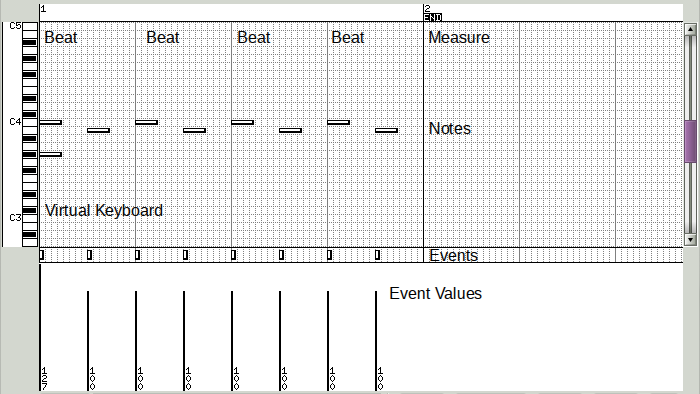
\includegraphics[scale=0.75]{pattern/pattern-edit-piano-roll-items.png}
   \caption{Pattern Editor, Piano Roll Items}
   \label{fig:pattern_editor_piano_roll_items}
\end{figure}

   \begin{enumber}
      \item \textbf{Beat}
      \item \textbf{Measure}
      \item \textbf{Virtual Keyboard}
      \item \textbf{Notes}
      \item \textbf{Events}
      \item \textbf{Event Values}
   \end{enumber}

   \setcounter{ItemCounter}{0}      % Reset the ItemCounter for this list.

   \itempar{Beat}{piano roll!beat}
   The light vertical lines represent the beats defined by the configuration
   for the pattern.  The even lighter lines between the beats are useful for
   snapping notes.

   \itempar{Measure}{piano roll!measure}
   The heavy vertical lines represent the measures defined by the
   configuration for the pattern.
   \index{pattern!end marker}
   Also note that the end of the pattern
   occurs at the end of a measure, and is marked by a blocky \textbf{END}
   marker.

   \itempar{Virtual Keyboard}{piano roll!virtual keyboard}
   The virtual keyboard is a fairly powerful interface.  It shows,
   by shadowing, which note on the keyboard will be drawn. It can be
   played with a mouse, using left-clicks, to preview a short motif.
   It can show marks to indicate off-scale notes, to make them easy to
   avoid.  Every octave, a note letter and octave number are shown, as in
   "C4".  If there is a difference scale in force, then the letter changes to
   match, as in "F\#5".

   \index{virtual keyboard!right-click}
   A right-click anywhere in the virtual keyboard area toggles the display
   between the octave note letters and the MIDI note numbers (only every other
   one is displayed due to space, to avoid cramped numbering).
   The following figure shows both views, superimposed for comparison.

\begin{figure}[H]
   \centering 
   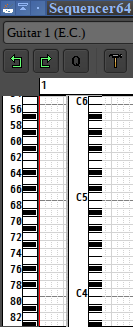
\includegraphics[scale=0.75]{pattern/pattern-edit-window-key-numbers.png}
   \caption{Pattern Editor, Virtual Keyboard Number and Note Views}
   \label{fig:pattern_editor_key_numbers}
\end{figure}

   \itempar{Notes}{piano roll!notes}
   Musical notes are indicated by thick horizontal bars with white
   centers.  Each bar provides
   a visual representation of the pitch of a note and the length of a note.

   \itempar{Events}{piano roll!events}
   \index{events pane}
   Also known as the "events pane" or "events panel".
   The small (just a few pixels high) events strip shows discrete events,
   such as Note On and Note Off and their velocities, or various Controller
   items and their values.  We recommend not editing or selecting events
   in that pane (feel free to disobey), but it is a good way to add events.
   Either
   \index{mouse!left-click}
   left-click (to add one event),
   \index{mouse!left-click-drag}
   or left-click-drag horizontally (to add a
   series of events at the current note resolution.)  One can also
   left-click in that section,
   \index{keys!p}
   then hit the \texttt{p} key to go into "paint" mode,
   \index{keys!x}
   and hit the \texttt{x} key to escape that mode.

   \itempar{Event Values}{piano roll!event values}
   Also known as the "data pane"
   \index{data pane}
   or "data panel".
   \index{data panel}

   The events values for the currently selected category of events are shown
   in this window as vertical lines of a height proportional to the value.
   These values can be easily modified by
   \index{mouse!left-click-drag}
   left-click-dragging the
   mouse past each line, to chop it off at the given value.  Easier to try
   it than explain it.
   \index{mouse!right-click-drag}
   Right-click-drag also works the same.

\subsubsection{Pattern Editor / Event Editing}
\label{subsubsec:seq64_pattern_editor_event_editing}

   When we say "editing" in the context of the piano roll, in part we mean that
   we will "draw" \index{draw mode}
   or "paint" \index{paint mode} notes.
   Drawing, modifying, copying, and deleting
   notes is actually very elegant in \textsl{Sequencer64} and in
   \textsl{Seq24}.

   Note editing is a bit different with \textsl{Sequencer64}, since it
   requires two mouse buttons in many cases.  There are some new
   laptop touchpads that really have only one mouse button, and
   use positioning to determine if the click is a left-click or a right-click.
   Two-fingered actions are devoted to scrolling, so that there is no way
   to generate a Linux middle-click.
   One solution is to use a four-button USB trackball
   configued with an easy middle-button setup.
   It's easier than a touchpad, anyway.
   So we've coded up a couple of solutions to this middle-click problem.

   Note that, if only a middle-button is needed,
   \texttt{Ctrl-left} will simulate that button.

%  Also note the "Mod4 mode" for the right-click action, and the
%  \texttt{p} and \texttt{x} keys for getting in and out of "paint mode",
%  discussed elsewhere.

   \textbf{New:}
   \index{keys!mod4}
   There is a feature to allow the Mod4
   \index{pattern editor!mod4}
   (the Super or Windows) key to keep the
   right-click in force even after it is released.  See \ref{new_mod4_mode}.
   Basically, pressing Mod4 before releasing the right-click that allows
   note-adding, keeps note-adding in force after the right-click is released.
   Now notes can be added at will with the left mouse button.  Right-click
   again to leave the note-adding mode.

   \textbf{New:}
   \index{new!paint mode}
   Another way to turn on the paint mode has been added.
   To turn on the paint mode, first make sure that the piano roll has the
   keyboard focus by left-clicking in it, then press the
   \index{keys!p}
   \texttt{p} key while in the sequence editor.
   This is just like pressing the right mouse button, but the draw/paint mode
   sticks (as if the Mod4 mode were in force).
   To get out of the paint mode, press the
   \index{keys!x}
   \texttt{x} key while in the sequence editor, to "x-scape" (get it? get it?)
   from the paint mode.
   These keys also work while the sequence is playing.

   The \texttt{p} and \texttt{x} keys also works in the small event strip just
   above the white data area.  The Mod4-right-click feature does not
   yet work in that aread of the user interface, but the \texttt{p} key does.

\paragraph{Editing Note Events}
\label{paragraph:seq64_pattern_editor_note_events}

   The Piano Roll pane provides for a quite sophisticated set of note-editing
   actions.  Not only is there a native mouse-interaction mode, but there is a
   "fruity" mouse-interaction mode that works more like the applications
   "Fruity Loops", it's follow-on "FL Studio', and its Linux look-alike,
   "LMMS".

   \setcounter{ItemCounter}{0}      % Reset the ItemCounter for this list.

   \itempar{Fruity Mode}{pattern editor!fruity mode}
   \index{todo!fruity mode}
   At some point, we will add a section detailing the usage of the "fruity"
   mode of mouse-interaction.

   Please study the following paragraphs carefully, ideally while
   trying them out in \textsl{Sequencer64}.

   \itempar{Enter Draw Mode}{pattern editor!draw mode}
   \index{pattern editor!right hold}
	In the note (grid/roll) panel, \textbf{holding}
	down the \textbf{right} mouse button will change the cursor
	to a pencil and put the editor into "draw" mode, 
   \index{draw mode}
   also known as "note-adding" or "paint" mode.
   \index{paint mode}
   To exit the draw mode, release the right mouse button, and the cursor will
   turn back into an arrow.

   Another way to enter paint mode is to make sure the piano roll has focus
   (left click in it), and then press the \texttt{p} key.
   To exit the draw mode, press the \texttt{Shift-p} key.

   \itempar{Add Notes}{pattern editor!add notes}
   \index{pattern editor!right hold left click}
   Then, while still \textbf{holding} the \textbf{right} mouse button, click
   the \textbf{left} mouse button to \textbf{insert} new notes.  Many people
   find this combination strange at first, but once one gets used to it, it
   becomes a very fast method of note manipulation.  An new option is to
   hold the Mod4 key while releasing the right button, which keeps the mouse
   in draw mode.  Another new option is to press the \texttt{p} to enter draw
   mode, and stay in it until \texttt{Shift-p} is pressed.
   \index{notes!inserting}
   Note that this click will add a single note, and the length of the note will
   be that specified in the note-length setting (e.g. "1/16").

   \index{pattern editor!right hold left drag}
   \index{notes!duration}
   To increase the number of notes, keep dragging the mouse (with
   both buttons held).  It can be dragged rightward, leftward, upward, and
   downward.
   \index{notes!auto}
   Dragging left or right adds new notes, while dragging upward or
   downward moves the current note to a different pitch.
   \index{auto-note}
   We call this the "auto-note" feature.
   Please note that the auto-note feature does \textsl{not} work with
   the chord-generation feature.

   The draw mode has the following features:

   \begin{itemize}
      \item Notes are continually added as the mouse is dragged ("auto-notes").
      \item Notes cannot be added past the "END" marker of the pattern, which
         marks the \textbf{Sequence Length in bars} setting.
      \item As the mouse is dragged while the left button is held in draw mode,
         notes are either added, or, if already present at that note-on time,
         are moved up and down.
      \item If the draw mode is exited, and entered again, then the original
         notes will not be altered.  Instead, new ones will be added.
      \item Notes can be added while the pattern is playing, and will be heard
         the next time the progress bar passes over them.
   \end{itemize}

   Thus, one can, with some care, draw a nice chorded sequence.
   Adjustments to it can be made afterward.

   \itempar{Select Notes}{pattern editor!select notes}
   Adjustments can be made to one or more notes by selecting one or more notes,
   and then applying one or more special
   \index{selection action} "selection actions" to the selection.

   \index{pattern editor!left click}
   \index{pattern editor!select note}
   \index{selection!single note}
   To select a single note, simply \textbf{left click} on it.
   The selected note will turn orange.

   \index{pattern editor!left click drag}
   \index{selection!multiple notes}
   To select multiple notes, perform a \textbf{left click drag}
   to form a selection box that intersects (even partly) the desired notes.
   Once the mouse is released, all of the desired notes should be orange.

   \index{pattern editor!ctrl left click drag}
   \index{selection!add multiple notes}
   To add more notes to a selection of notes, move to an unselected note
   and perform a \textbf{ctrl left click drag}
   to form a selection box that intersects (even partly) the desired notes.
   Once the mouse is released, all of the desired notes should be orange.
   Be careful!  If you ctrl-left-click-drag on an already-selected note,
   the drag will change the length of all of the notes in the selection.

   \index{keys!ctrl-a}
   \index{selection!all}
   Pressing the \texttt{Ctrl-A} key will select all of the events in the
   pattern editor.

   The \textbf{Tools} button described in
   \sectionref{subsec:seq64_pattern_editor_second} can also be used to
   modify selections.

   Once one or more notes are selected, they can be modified in time,
   pitch, or length.

   \itempar{Deselect Notes}{pattern editor!deselect notes}
   \index{selection!deselect}
   To deselect the notes, click somewhere else in the piano roll, and the notes
   should change back to white.

   There is no way to deselect a single note, with, say a shift-click
   or ctrl-click action.

%  \index{notes!lengthen}
%  For example, if one wants a long single note, first draw the
%  short note, and then use one of the operations described in the next
%  paragraph to change the length of the note.  These operations also cause
%  the note to be selected.

   \itempar{Move Notes in Pitch}{pattern editor!move notes in pitch}
   To move notes in pitch, once selected, grab one of the notes in the
   selection and drag it upward or downward.
   \textbf{New:}
   \index{new!down arrow}
   \index{new!up arrow}
   Also, since a selection is in force, the Up and Down arrow keys can also
   be used to change the pitch of every note in the selection.
   The smallest unit of pitch change is one MIDI note value.

   \textbf{Warning:}
   \index{warning!down arrow}
   \index{warning!up arrow}
   \index{warning!note loss}
   If one moves the selection too low or too high in pitch, whether with the
   mouse or the arrow keys, any notes that go below the lowest MIDI pitch or
   above the highest MIDI pitch \textbf{will be lost}!
   If done using the mouse, the undo feature (Ctrl-z) will work.
   If done using the arrow keys, the undo feature does not work!
   Be careful, especially if you have a fast keyboard repeat rate!

   \itempar{Move Notes in Time}{pattern editor!move notes in time}
   To move notes in time, once selected, grab one of the notes in the
   selection and drag it leftward or rightward.
   \textbf{New:}
   \index{new!left arrow}
   \index{new!right arrow}
   Also, since a selection is in force, the Left and Right arrow keys can also
   be used to change the time of every note in the selection.
   The smallest unit of time change is the \textbf{Grid snap} value,
   which might be a 16th note, for example.

   Note that there is no possibility of note loss with a change in time.  When
   a note disappears at one end of the pattern boundary, it wraps around to the
   other end.  Cool.

   (There is another feature of the arrow keys when no selection is made, that
   supposedly moves an "origin" for playback, but we haven't been able to
   figure out exactly if it does anything.)

   \itempar{Change Note Length}{pattern editor!change note length}
   \index{pattern editor!ctrl left click drag}
   \index{pattern editor!middle click drag}
   Pressing the \textbf{middle} mouse button \textbf{\textsl{or}}
   pressing the \textbf{ctrl left} mouse button in tandem, while the pointer is
   hovered over a selected note, will let one
   \index{notes!duration change}
   change the length of a selected note.  If more than one note is selected,
   then the length of all selected notes is changed.

   \index{pattern editor!event stretch}
   \index{pattern editor!shift middle click drag}
   \index{event!stretch}
   \index{stretch events}
   Once a selection of notes is made, one can use the
   shift-middle-click-drag (true?) or ctrl-left-click-drag
   sequence over the selected notes to
   draw a box beyond the extent of the notes.  When the mouse is released,
   each of the events is moved and lengthed to be proportionally longer to
   fit exactly within the box one drew.
   This feature is called \textsl{event stretch}.

   \index{pattern editor!event compression}
   \index{event!compression}
   \index{compress events}
   If the box that was drawn was shorter than the original extent of the
   notes, then the notes move and shrink proportionally to occupy the
   smaller box.
   This feature is called \textsl{event compression}.
   
   \index{warning!wrap-around notes}
   \textbf{Warning}:  If one reduces or increases the length of a note selection
   by too much, the note or notes will "wrap-around" to the end of the sequence
   boundary and grow more from the beginning of the sequence. 
   It is not clear if this new note has an ending time that is less than its
   beginning time.  If it happens, one probably ought to undo it.

   Note that notes can be shortened below the default note length by event
   compression.  Note that there is currently no way to change the length of
   the note using a keystroke.

   \itempar{Copy/Paste}{pattern editor!copy/paste}
   Copying, cutting, and pasting is supported by selecting a number of events
   or notes, and using the
   \index{pattern editor!cut}
   \index{keys!ctrl-x} Cut (\texttt{Ctrl-X}), 
   \index{pattern editor!copy}
   \index{keys!ctrl-c} Copy (\texttt{Ctrl-C}),
   \index{pattern editor!paste}
   \index{keys!ctrl-v} Paste (\texttt{Ctrl-V}), and
   "drop" (\texttt{Enter})
   \index{pattern editor!drop}
   \index{keys!enter}
   keys.
   When the notes are selected,
   \index{pattern editor!delete}
   \index{keys!del}
   \index{keys!backspace}
   one can delete them with the \texttt{Delete} or \texttt{Backspace} key.
   If the events are \textsl{cut}, using the \texttt{Ctrl-X} key, then
   they can be pasted, using the \texttt{Ctrl-V} key.  However,
   once \texttt{Ctrl-V} is struck, then one must \textsl{move} the mouse
   pointer to see where to paste the events, or move it with the arrow keys.
   An orange box representing the
   selected-and-copied notes appears, and the user should move the box (note)
   to the desired location and then left-click.

   \textsl{
   (Warning:  We've had temporary issues where the selection box flickers, and
   this seems to be due to updates in the graphics library used by
   \textsl{Sequencer64}.  This issue might depend on the Linux distro one
   uses.)
   }

   Additionally, one can move the orange box using the arrow keys, to the
   desired location, and then hit the
   \index{keys!enter} \texttt{Enter} key to
   drop the notes at that location.

   Finally, note that selected notes that are cut or copied can then be
   pasted into \textsl{other} pattern editor dialogs; that is, they can be
   pasted into other sequences.

\begin{figure}[H]
   \centering 
   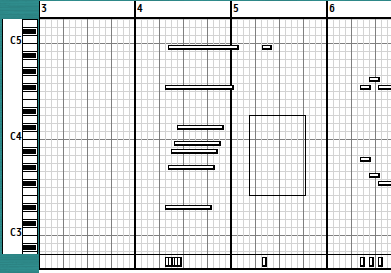
\includegraphics[scale=0.75]{pattern/selection-paste-box.png}
   \caption{Piano Roll, Paste-Box for Cut Notes}
   \label{fig:pattern_editor_selection_paste_box}
\end{figure}
   
   Note that the selection box is now orange, not black.
   Move this box to where pasting is
   desired, and left-click.  The moved notes appear, still selected,
   and they can then be moved further, if desired, by using the arrow keys, or
   cut and move them again.

   For the appearance of selected events (orange), see
   \figureref{fig:pattern_editor_selected_events}.

\begin{figure}[H]
   \centering 
%  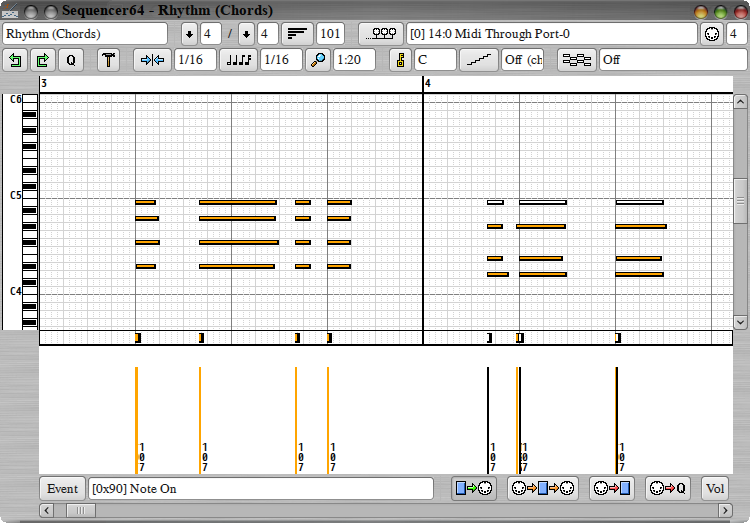
\includegraphics[scale=0.75]{pattern/pattern-edit-selected-events-0-9-10.png}
   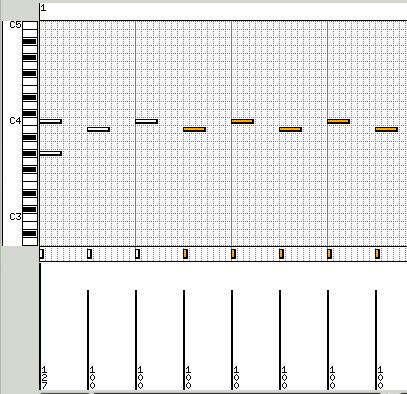
\includegraphics[scale=0.75]{new/pattern-edit-selected-events.png}
   \caption{Piano Roll, Selected Notes and Events}
   \label{fig:pattern_editor_selected_events}
\end{figure}

   \textbf{New:}
   \index{new!selected data coloring}
   The selection, shown in
   \figureref{fig:pattern_editor_selected_events},
   illustrates the new style of event selection, which colors the data
   bars as well as the event and note bars.  This selection was made by first
   selecting one set of events by the
   \index{mouse!left-click-drag}
   left-click-drag action, then
   \index{mouse!ctrl-left-click-drag}
   selecting more events by holding the Ctrl key for the next left-click drag
   action.  The second selection left out some events, which are thus still
   shown as black bars in the data area.

   As an aside, note that the event strip is gray.  \textsl{Sequencer64}
   now shows this strip as gray when the selected event (the \textbf{Event}
   button) is Note On, Note Off, or Aftertouch.  This color is purely a
   reminder that moving these events can really screw up the notes, for example
   by moving Note Off to before the Note On event.
   
\paragraph{Editing Other Events}
\label{paragraph:seq64_pattern_editor_other_events}

%  Left-click or right-click on events in the event strip (directly under
%  the piano roll grid) will allow one to add/select/move 
%  MIDI events (including note on/off messages) somewhat like the 
%  piano grid.

   \index{event strip}
   \textsl{Note On} and \textsl{Note Off} events (and other events) can appear
   as small squares in the event strip, along with a black vertical bar with a
   height proportional to the velocity of the note event, plus a numeric
   representation of that value.
   Note events do not need to be inserted in the event strip.
   \index{warning!unterminated notes}
   (\textsl{Note events can be inserted there, but they end up as short
   events of the lowest possible note, 0 or C1, and they don't have a Note
   Off event.  So don't do that!})

   \index{events!insert}
   Other event types can be inserted via the event strip.  To do that, first
   select the kind of event to insert using the \textbf{Event} button in the
   bottom panel.  The place the mouse cursor in the event strip.
   Right-click to make the drawing pencil appear at the exact spot where the
   event must go.  While holding the right button, click the left button.
   A small square for the event should appear.

   Should one want more of the same event, continue to hold both buttons and
   drag the mouse.  One event should appear at each beat position (e.g. at
   each 16th note position) that is crossed.

   To move the event(s) to a different spot, select it or them via the left
   button.  Then drag it or them to where one wants them.
   \index{todo!high precision events}
   it is currently not possible to move them to positions smaller than the
   beat size.  The work-around is to temporarily reduce the beat size,
   but this requires caution.

   Once the event positions are set, the next step is to modify the
   data values of the events.

   \index{event data}
	The event value (data) editor (directly under the event strip) is used 
	to change note velocities, channel pressure, control codes,
	patch select, etc.
   \index{event data editor!draw}
   \index{event data editor!left click}
   \index{event data editor!right click}
   \index{event data editor!middle click}
   Just left-click+drag the mouse across the window to draw a line.  The
   values will match that line.  
   middle-click+drag and right-click+drag also
   draw the value line.

   \textbf{Bug:}
   \index{bugs!event editing can fail}
   Sometimes the editing of event values in the event data section will not work.
   The workaround is to do a \texttt{Ctrl-A}, and the click in the roll
   to deselect the selection; that makes the event value editing work again.
   
   \index{event data editor!mouse wheel}
   Any events that are selected in the piano roll or event strip can have
   their values modified with the mouse wheel.

\paragraph{Editing Note Events the "Fruity Way"}
\label{paragraph:seq64_pattern_editor_note_events_fruity}

   This mode is a lot different, and we have yet to do the exhaustive testing
   needed to understand how this mode works.  Input from actual users of this
   mode would be welcome.

\subsection{Pattern Editor / Bottom Panel}
\label{subsec:seq64_pattern_editor_bottom}

   The bottom horizontal panel of the Pattern Editor provides for
   selecting events for viewing and edition, and the MIDI playback,
   pass-through, and recording options of \textsl{Sequencer64}.

\begin{figure}[H]
   \centering 
   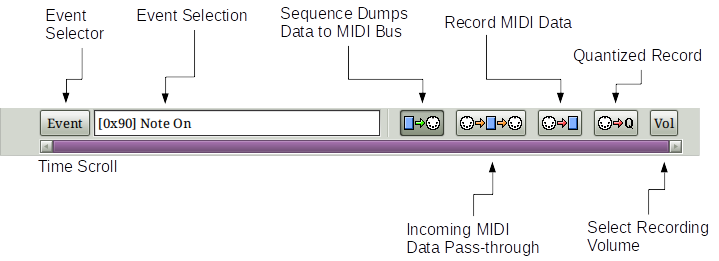
\includegraphics[scale=0.75]{pattern/pattern-edit-bottom-panel-items.png}
   \caption{Pattern Editor, Bottom Panel Items}
   \label{fig:pattern_editor_bottom_panel_items}
\end{figure}

   Until we can get a completely labelled screenshot, here is the
   latest bottom panel, with the new \textbf{LFO}
   and \textbf{Recording Type} buttons, and the popup menu for the latter.

\begin{figure}[H]
   \centering 
   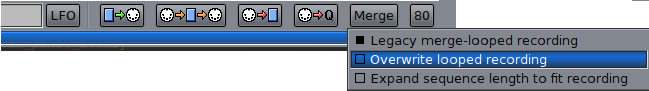
\includegraphics[scale=0.75]{new/lfo_and_rectype_buttons.png}
   \caption{Pattern Editor, Additional Bottom Panel Items}
   \label{fig:pattern_editor_added_bottom_panel_items}
\end{figure}

   \begin{enumber}
      \item \textbf{Event Selector}
      \item \textbf{Event Selection}
      \item \textbf{LFO} (if built with LFO support; not shown)
      \item \textbf{Time Scroll}
      \item \textbf{Data To MIDI Buss}
      \item \textbf{MIDI Data Pass-Through}
      \item \textbf{Record MIDI Data}
      \item \textbf{Quantized Record}
      \item \textbf{Recording Type} (Merge, Replace, Expand)
      \item \textbf{Select Recording Volume}
   \end{enumber}

   \setcounter{ItemCounter}{0}      % Reset the ItemCounter for this list.

   \itempar{Event Selector}{pattern editor!event selector}
   This button brings up the following context menu, so that the user can
   select the category of events to view and edit.

\begin{figure}[H]
   \centering 
   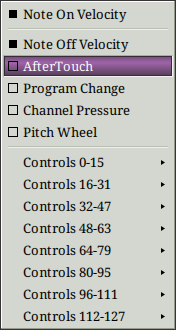
\includegraphics[scale=0.75]{pattern/event-context-menu.png}
   \caption{Pattern Editor, Event Button Context Menu}
   \label{fig:pattern_editor_bottom_event_context_menu}
\end{figure}

   The sub-menus of this context menu show 128 controller messages,
   so we won't try to show all of them here.

   These sub-menus can be modified, as far as we know, by editing
   the file
   
   \begin{verbatim}
      $HOME/.config/sequencer64/sequencer64.rc
   \end{verbatim}

   (legacy mode: \texttt{\$HOME/.seq24usr}), to make it match one's
   instrument.  See \sectionref{sec:seq64_usr_file}.

   \itempar{Event Selection}{pattern editor!event selection}
   Shows the selection event, with its number shown in hexadecimal notation,
   and the name of the event shown.

   \textbf{New:}
   \index{new!LFO control}

   \itempar{LFO}{pattern editor!LFO}
   If \textsl{Sequencer64} is built with the \texttt{--enable-lfo} option,
   then a low-frequency oscillator functionality is built so that data events
   can be modulated by some rudimentary wave functions.
   This feature is now enabled by default.
   By clicking on the \textbf{LFO} button or using the \texttt{Ctrl-L} key,
   the following window appears:

\begin{figure}[H]
   \centering 
   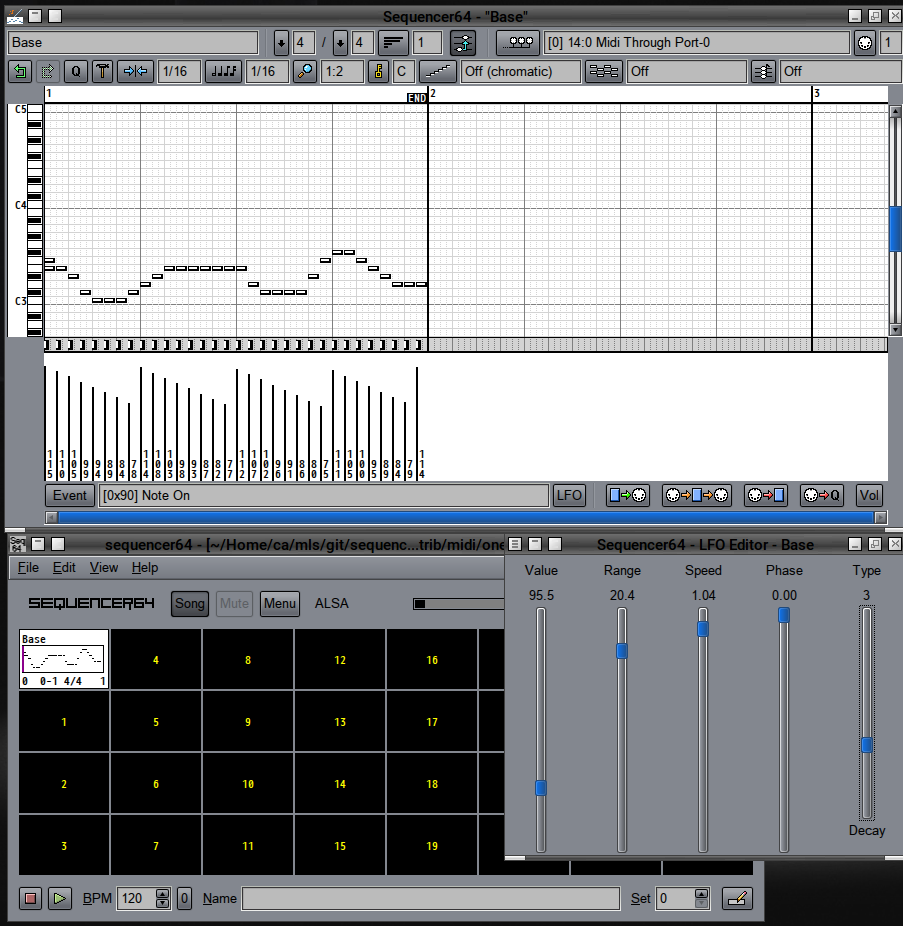
\includegraphics[scale=0.75]{new/pattern_editor_with_LFO.png}
   \caption{Pattern Editor, LFO Support}
   \label{fig:pattern_editor_bottom_lfo_support}
\end{figure}

   Note the controls in this window:

   \begin{enumber}
      \item \textbf{Value}:
         Provides a kind of DC offset for the data value. Starts at 64, and
         ranges from 1 to 127.
      \item \textbf{Range}:
         Controls the depth of modulation. Starts at 64, and ranges from 1 to
         127.
      \item \textbf{Speed}:
         Indicates the number of periods per pattern (divided by beat width,
         normally 4).  For long patterns, this parameter needs to be set high,
         to even show an effect.  It is also subject to an 'anti-aliasing'
         effect in some parts of the range, especially for short patterns.
         Try it!  For short patterns, try a value of 1 at first.  For a pattern
         of one measure in length, this will create four periods of the wave.
      \item \textbf{Phase}:
         Provides the phase shift within a period of the LFO wave.
         A value of 1 is a phase shift of 360 degrees (or maybe it is one
         radian?).
      \item \textbf{Wave Type}:
         Selects the kind of wave to use for the LFO:
         \begin{enumber}
            \item \textbf{Sine wave}.
            \item \textbf{Ramp (up) sawtooth}.
            \item \textbf{Decay (down) sawtooth}.
            \item \textbf{Triangle wave}.
         \end{enumber}
   \end{enumber}

   We may have more to explain about this dialog at some point.  For now,
   try it out on the file \texttt{one-measure.midi}, and be sure to hover over
   each control to see the tooltips.
   Note that it works best with short patterns.

   \itempar{Time Scroll}{pattern editor!time scroll}
   Allows one to pan through the whole pattern, if it is too long to fit in
   the window horizontally.

   \itempar{Data To MIDI Buss}{pattern editor!data to midi buss}
   Activating this button will cause the pattern to be output to the MIDI
   output buss, which will normally be connected to a software or hardware
   synthesizer, to be heard.
   Generally, this control should always be activated.

   \itempar{MIDI Data Pass-Through}{pattern editor!midi data pass-through}
   Activating this button will route incoming MIDI data through
   \textsl{Sequencer64}, which will then write it to the MIDI output buss.

   \itempar{Record MIDI Data}{pattern editor!record midi data}
   Activating this button will route incoming MIDI data into
   \textsl{Sequencer64}, which will then save the data to its buffer, and also
   display the new information (notes) in the piano roll view.

   \itempar{Quantized Record}{pattern editor!quantized record}
   Activating this button will also cause MIDI data to be recorded, but it
   will be quantized on the fly before recording it.

   \itempar{Recording Type}{pattern editor!recording type}
   In \textsl{Seq24}, the pattern recording worked by merging new notes played
   as the pattern to be recorded was looped.  This method allows a loop to be
   built up bit-by-bit.  \textsl{Sequencer64} adds two more methods from
   Stazed's \textsl{Seq32} project.  The three methods are:

   \begin{enumber}
      \item \textbf{Merge}. \index{merge}
      \index{recording type!merge}
      This is the "legacy" style of recording loops, where notes can
      accumulate.
      \item \textbf{Replace.} \index{replace}
      \index{recording type!replace}
      In this method of recording, whenever the loop starts over, and a note is
      pressed, then the existing notes in that loop are erased, and the new
      note is added.  This provides a good way of correcting major mistakes,
      live.  Note that this method will not work if adding notes while not
      recording.
      \item \textbf{Expand}. \index{expand}
      \index{recording type!expand}
      In this method of recording, once the end of the loop is nigh, whether or
      not any notes are being input, another measure is added to the length of
      the loop.  This continues indefinitely, whether or not any notes are
      being recorded.
   \end{enumber}

   \itempar{Vol}{pattern editor!vol}
   This button allows controlling the volume of the recording.
   The velocity of the notes will be set to the selected value upon recording.
   If the \textbf{Free} item is selected, then the incoming note velocity is
   preserved.

\begin{figure}[H]
   \centering 
   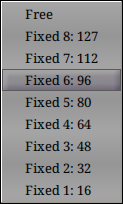
\includegraphics[scale=0.75]{pattern/vol-context-menu-new.png}
   \caption{Pattern Recording Volume Menu}
   \label{fig:pattern_edit_recording_volume_menu}
\end{figure}

   The values provided are:

   \begin{itemize}
      \item Free (record incoming volumes).
      \item Fixed 8, Fixed 7, Fixed 6, Fixed 5, Fixed 4, Fixed 3.
      \item Fixed 2, and Fixed 1.
   \end{itemize}

   These values correspond to MIDI volume levels from 127 down to 16, as
   shown in the figure.

   One thing fixed in the 0.90.x version is the ability to store MIDI note-on
   events with the actual velocity provided by the MIDI keyboard used to
   generate the notes.  Previously, even in \textsl{seq24},
   the \textbf{Free} option in the \textbf{Vol} menu option did not work.
   This is fixed.

\subsection{Pattern Editor / Common Actions}
\label{subsec:seq64_pattern_editor_common}

   This section is a catch-all for actions not described above.

\subsubsection{Pattern Editor / Common Actions / Scrolling}
\label{subsec:seq64_pattern_editor_scrolling}

   Let us describe the actions that can be performed with a
   scroll wheel, or with the scrolling features of multi-touch touchpads.
   There are three major scrolling actions available when using mouse
   scrolling, with the mouse hovering in the piano-roll area:

   \begin{itemize}
      \item \textbf{Vertical Panning (Notes Panning)}
         \index{scroll!normal scroll}
         \index{scroll!vertical pan}
         \index{scroll!notes pan}
         \index{pan!seqroll notes}
         Using the vertical scroll action of a mouse or touchpad moves the
         view of the sequence/pattern notes up and down.
         One can also click in the piano roll, and then use the
         \texttt{Page-Up} \index{keys!page-up}
         and \texttt{Page-Down} \index{keys!page-down}
         keys to move the view up and down in pitch.
      \item \textbf{Horizontal Panning (Timeline Panning)}
         \index{scroll!shift scroll}
         \index{scroll!horizontal pan}
         \index{scroll!timeline pan}
         \index{pan!seqroll time}
         Holding the Shift key, and then using the vertical scroll action of a
         mouse or touchpad moves the view of the sequence/pattern time forward
         and backward.
         One can also click in the piano roll, and then use the
         \texttt{Shift Page-Up} \index{keys!shift page-up}
         and \texttt{Shift Page-Down} \index{keys!shift page-down}
         keys to move the view left and right in time.
      \item \textbf{Horizontal Zoom (Timeline Zoom)}
         \index{scroll!ctrl scroll}
         \index{scroll!horizontal zoom}
         \index{scroll!timeline zoom}
         \index{zoom!seqroll time}
         Holding the Ctrl key, and then using the vertical scroll action of a
         mouse or touchpad zooms the view of the sequence/pattern time to
         compress it or expand it.
         One can also click in the piano roll, and then use the
         \texttt{z} \index{keys!z},
         \texttt{Z} \index{keys!Z}, and
         \texttt{0} \index{keys!0} to change the timeline zoom.
   \end{itemize}

   The actions of this scrolling are surprisingly smooth and fast.
   If an event is selected in the piano-roll area or the (thin) event area,
   then the scrolling action increases or decreases the value of the event.
   In the case of a note, this increases or decreases the velocity of the note.
   For all events, this increases or decreases the length of the vertical line
   that represents the value of the event.

\subsubsection{Pattern Editor / Common Actions / Close}
\label{subsec:seq64_pattern_editor_close}

   There is no \textbf{Close} button in the pattern editor.  One can use
   window-manager actions, such as clicking on the X button of the window
   frame, or pressing the exit key defined in the window manager.

   \textsl{Sequencer64} also provides the Ctrl-W key to close the pattern
   editor window.
   \index{window!close}

   However, be aware that this convention does not apply to the other
   application windows of \textsl{Sequencer64}.

%-------------------------------------------------------------------------------
% vim: ts=3 sw=3 et ft=tex
%-------------------------------------------------------------------------------
